
%3/4 pages au moins en français (idem pour conclusion)
%\begin{itemize}
%\item fines échelles et leur rétroaction/structuration de circu générale
%\item choix région Gibraltar (Rencontre deux masses d'eaux, alimentation Méditerranée, outflow med)
%\item les fines échelles à Gibraltar (quels phénomènes (solitons, ressaut, etc))
%\item Outils de la thèse : num, obs (compagne,sat)
%\item état des lieux modélisation num fines échelles océaniques, problematique quantification mélange diapycnale
%\item plan
%\end{itemize}

Certains des éléments bibliographiques sont repris dans les introductions des différents chapitres, conçus comme des articles.

\section[Un voyage en \textit{Terra incognita}]{Un voyage en \textit{Terra incognita\footnote{\cite{scotti_large_2010}}}}
\subsection{Dynamique océanique : vers les fines échelles}
\label{subsection_intro1}
%(pose principes circu océanique, présente contexte des échelles généralement considérées en océanographie physique)

%La circulation globale océanique, pilotée par les vents et le flux de flottabilité, s'organise en un ensemble de courants de grande échelles (gyre, AMOC,...) qui en parallèle et en interaction avec la dynamique de l'atmosphère, transporte la chaleur. \\
\begin{figure}[!h]
  \centering
  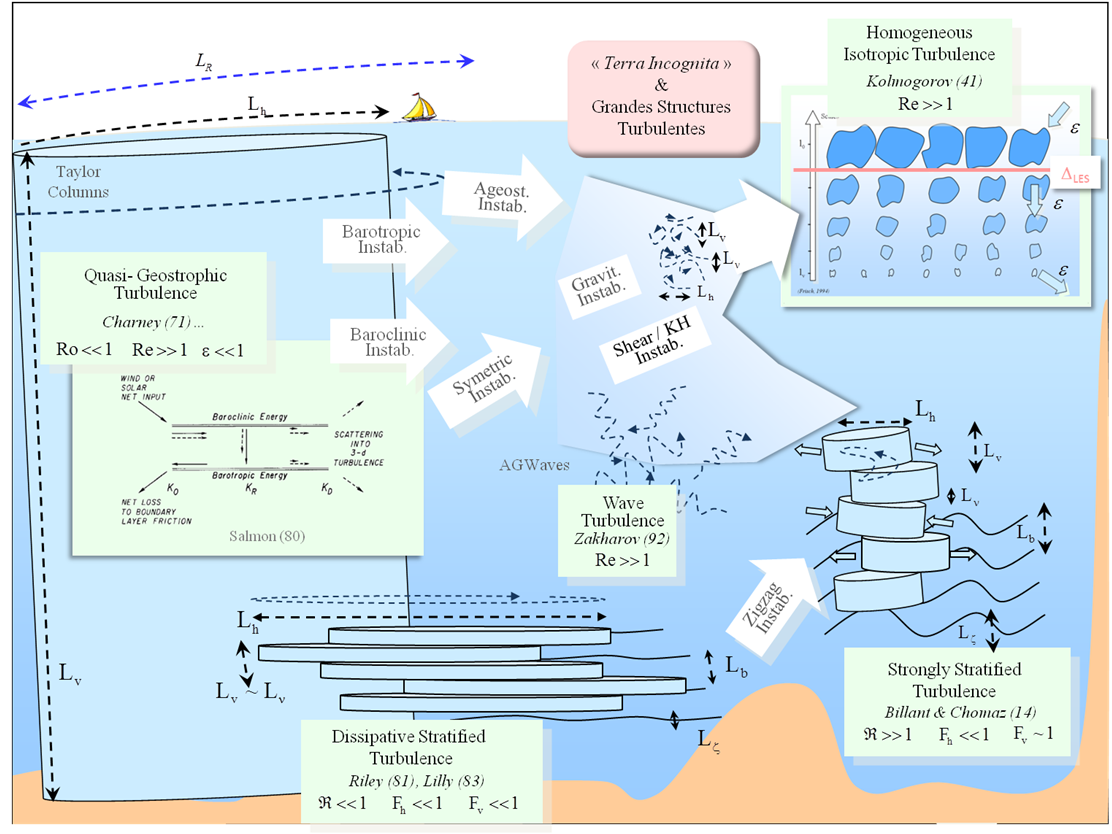
\includegraphics[width=0.8\textwidth]{./INTRO/Ocean_scales.png}
  \caption{\color{red}l'océan vu à travers ses cascades d'échelles, ses instabilités et ses principaux modèles de turbulence.\color{black}}
  \label{fig_ocean_scales}
\end{figure}
%\color{blue}
L'océan est soumis à/ mis en mouvements sous l'action de nombreux forçages par la pression atmosphérique, les marées astronomiques ou les flux de quantité de mouvement induits par le vent mais aussi par les flux de chaleur radiatifs ou par les flux de chaleur latente ou encore par les précipitations, les fleuves ou encore par évaporation... Ainsi présenté, l'océan peut donc être présenté comme un \textit{système dynamiquement ouvert}, l'ensemble des forçages auxquels il est soumis induisant un large spectre de processus dynamiques: houle, courants d'Ekman, upwelling ou downwelling, ondes de marée, marées internes, convection profonde, courants de gravité, panaches fluviaux... 


La dynamique de l'océan est variée, composée de processus dynamiques couvrant une large gamme autant spatiale que temporelle. La houle, les courants d'Ekman, les systèmes d'upwelling ou de downwelling, les ondes de marée, les marées internes, la convection profonde, les courants de gravité, ou encore les panaches fluviaux, 

, composée d'une large gamme de processus aux extensions géographiques 


%d'un large spectre de processus, on peut citer la houle, les courants d'Ekman, les systèmes d'upwelling ou de downwelling, les ondes de marée, les marées internes, la convection profonde, les courants de gravité, ou encore les panaches fluviaux... 

L'océan ne se résume toutefois pas à une somme de processus "forcés" dont la combinaison linéaire suffirait à expliquer sa dynamique propre. Ces processus interagissent en effet entre eux induisant d'importants \textit {mécanismes de transferts} entre les différentes gammes d'échelles spatiales et temporelles. Lorsque ces transferts prennent une forme cohérente dans quelques régions spécifiques du spectre, on parle de \textit{cascades d'échelles}. Les mécanismes débouchant sur ces transferts sont quant-à eux généralement associés à des \textit{instabilités dynamiques}.\\
\cite{salmon_baroclinic_1980} montrent par exemple qu'à méso-echelle\footnote{Région du spectre constitué d'échelles plus grande que le premier rayon de Rossby.} ces transferts s'organisent de façon cohérente sous la forme d'une \textit{cascade inverse} associée à des transferts énergétiques barotropes dirigés majoritairement vers les plus grandes échelles\footnote{Une telle cascade "inverse" est caractéristique de régimes de turbulence 2D.} alors que les transferts d'enstrophie\footnote{A l'image de l'énergie cinéatique cinétique pour la vitesse, l'enstrophie est définie comme la moitié du carré de la vorticité relative, i.e. du rotationnel de la vitesse.} sont quant à eux majoritairement dirigés vers les plus fines échelles. 
Les vents et les flux de chaleur induisent ainsi des structures dynamiques (baroclines) qui sont brisées lorsque l'écoulement devient instable \citep{vallis_atmospheric_2006}.
Les \textit{instabilités barotropes et baroclines} sont par conséquent au coeur de cette cascade dite inverse, elles rythment les transferts autour des rayons de Rossby\footnote{Échelle caractéristique de longueur caractérisant localement l'impact de la rotation du globe terrestre sur une colonne océanique de stratification donnée.} barotropes et baroclines dans les écoulements de mésoéchelles. On parle de régime de \textit{turbulence géostrophique} \citep{charney_geostrophic_1971} dans une région du spectre où stratification de la colonne d'eau et rotation du globe terrestre jouent \textit{in fine} des rôles prépondérants et sont associés à des équations de bilan équilibrées de quantité de mouvement. La cascade inverse demeure toutefois un modèle qualitatif fournissant une grille de lecture pour processus complexes et "non localisés" du le spectre océanique.\\
Des structures de sous-mésoéchelle reçoivent ainsi énergie et enstrophie et sont elles-aussi sujettes à un large éventail d'instabilités \citep{mcwilliams_submesoscale_2016}: instabilité agéostophique, symétrique, frontale, convective ou encore instabilités de cisaillement, instabilités baroclines dans la couche de mélange océanique, instabilités paramétriques des ondes internes... Dans cette région du spectre, l'impact de la rotation du globe terrestre est plus faible qu'à mésoéchelle mais la stratification contraint fortement la dynamique océanique débouchant sur des formes de turbulence dites "stratifiées": \textit{turbulence stratifiée dissipative}, \textit{turbulence fortement stratifiée}. l'instabilité "zig-zag" fait office de pont entre ces deux formes de turbulence).\\
Les myriades d'ondes de gravité internes et d'ondes de gravité de surface interagissent aussi au point de donner lieu à une forme particulière de turbulence: \textit{la turbulence d'onde}. Leur déferlement, leurs instabilités donnent généralement naissance à des "patchs turbulents" annoncés par l'apparition de grandes structures turbulentes.\\
En deçà de cette mésoéchelle (on parle de sous-mésoéchelle), prend naissance une autre cascade présentant une certaine cohérence, la \textit{cascade directe} ou cascade de Richardson au sein de laquelle l'énergie est transférée "directement" vers l'échelle de Kolmogorov au delà de laquelle la dissipation moléculaire est active. Si les théories décrivant les transferts à mésoéchelles ne permettent pas de routes directes vers la dissipation, les transferts de sous-mésoéchelle le permettent.
Les \textit{grandes structures turbulentes} marquent l'entrée de cette cascade directe, elles sont associées à des instabilités de cisaillement telles que les instabilités de Kelvin-Helmholtz. A \textit{micro-échelle}, le modèle de turbulence homogène et isotrope 3D décrit de façon simple cette cascade. Les échelles spatiales et temporelles des grandes structures turbulentes ne sont toutefois pas clairement définies: elles peuvent atteindre quelques dizaines de mètres au sein de la colonne d'eau mais peuvent aussi ne pas dépasser le mètre dans les couches de surface ou de fond.\\
Cascades d'échelles et modèles de turbulence décrivent ainsi des régions spécifiques du spectre spatio-temporel de l'océan qui présentent une certaine cohérence. Les divers types d'instabilités tissent quant-à elles des ponts entre ces régions. En toute rigueur, comprendre, expliquer, simuler (explicitement) ou modéliser (implicitement) le mélange turbulent, impliquent donc évidemment de représenter correctement l'ensemble du spectre océanique, ses transferts, ses cascades... Elle requière toutefois plus spécifiquement de reproduire précisément la cascade turbulente directe, i.e. le transfert "inertiel" d'énergie aboutissant à la région "dissipative" du spectre. Le point de départ de cette cascade n'est cependant pas clairement défini et varie aussi bien dans le temps que dans l'espace. Seule l'apparition souvent intermittente de grandes structures turbulentes permet de localiser spatialement et temporellement ce point de départ.\\
%Les grandes structures turbulentes marquent donc l'entrée de la cascade directe menant à la dissipation moléculaire. Elles sont ainsi à l'origine d'une cascade débouchant sur une réorganisation irréversible, diabatique de la colonne d'eau et d'un redistribution des "traceurs" passifs ou actifs. Parmi ces "traceurs", la masse volumique joue un rôle particulier dans la dynamique océanique: les masses d'eau sont par exemple "transportées" le long des surfaces isopycnales et le contenu en vorticité potentielle entre deux de ces surfaces isopycnales se conserve au cours du temps.\\
A. Scotti \citep{scotti_large_2010}, dans une revue sur la modélisation de l'océan, conclut qu’avec l'étude des grandes structures turbulentes, s'ouvrent les portes de la \textit{terra incognita}. Il reprend ainsi la conclusion de J.C. Wyngaard \citep{wyngaard_toward_2004} rédigée quelques années auparavant pour l'atmosphère. Cette terre inconnue, souvent aussi qualifiée de "zone grise" abritant les \textit{fines échelles océaniques}, est plus largement considérée comme la région particulièrement mal connue du spectre océanique dans laquelle la dynamique peut localement et temporairement basculer d'un équilibre simple entre un nombre limité de processus vers une dynamique non-linéaire complexe induisant une cascade d'instabilités dynamiques (directe) aboutissant à la dissipation moléculaire. 
\color{black}
%Cependant, l'océan (tout comme l'atmosphère) a un écoulement turbulent, c'est-à-dire chaotique et non-linéaire/ constitué d'une intéraction d'échelle.
%...
%Cette turbulence se manifeste en la décomposition des structures de grande échelles/synoptiques en des champs de plus petite structures/structures de plus en plus petites (transiant?) en intéractions les unes avec les autres (tourbillons, etc). Ainsi l'étude de l'océan peut se faire à bien des échelles spatiales et temporelles
%Ce manuscrit de thèse porte sur l'étude d'une dynamique dite de 'fine échelle', sur les processus / phénomènes océaniques . Il s'agira 
\color{blue}
\subsection{Rétroactions}
\label{subsection_retroactions}
Le mélange peut ainsi être présenté comme l'aboutissement de transferts et de cascades plus ou moins cohérentes mais quoiqu'il en soit très hétérogènes et intermittentes. Il ne constitue toutefois pas un puits sans fond ou un aller sans retour. Les flux diapycnaux modifient en effet les masses d'eau, la dissipation visqueuse qui "injecte" de la vorticité potentielle\footnote{La vorticité potentielle est une quantité, une substance d'après \cite{haynes_conservation_1990}, essentielle dans la description des écoulements stratifiés et en rotation qui est conservée par advection} près du fond... et constituent donc autant d'exemples de retroaction sur la grande échelle.\\
\cite{penney_2020} ont montré que le mélange était finalement capable de structurer les plus grandes échelles en mettant en évidence l'apparition à plus grande échelle de relations linéaires entre la masse volumique et les traceurs passifs qu'ils simulent.\\
La région du détroit de Gibraltar séparant la mer Méditerranée de l'océan Atlantique est à ce titre tout à fait exemplaire. Les masses d'eau méditerranéennes et atlantiques s'y croisent de façon tout aussi éphémère que brutale. Le mélange de ces deux masses d'eau induit par les fortes amplitudes de marée modifient in fine la salinité ou la quantité de mouvement de ces masses d'eau exerçant un contrôle sur la dynamique de l'ensemble du bassin Méditerranéen \citep{armi_1988}, scellant en quelques sortes le régime dynamique de l'ensemble du bassin et fixant vraisemblablement le contenu en vorticité potentielle du jet méditerranéen en Atlantique Nord.\\
La dissipation turbulente exerce donc une rétroaction sur les plus grandes échelles du spectre océanique: elle  structure les masses d'eau mais aussi la circulation océanique.
\color{black}
%(Revient plus en détail sur la turbulence, cas où mot est utilisé (turbulence géostrophique? vs cascade turbulente))
%Turbulence de mésoéchelle (instabilité barocline), ici on s'intéresse au début de la cascade turbulente directe définie par Kolmogorov. Les 2 sont similaires en ce qu'elles concernent le transfert d'énergie vers de plus fines échelles. Pour le cas de la turbulence de fine échelle, // mais va aussi aboutir à structuration de l'écoulement en lui-même. (La conservation de la vorticité potentielle (PV) peut agir comme un effet structurant de jet/courants...//méandres d'un jet / courant structurés par la conservation de la vorticité potentielle... PV générée par diabatic processes (in boundary layers?)...

%Cascade inverse???

\subsection{Le détroit de Gibraltar}
%(intérêt de la zone en vu du blabla précédent)
\color{blue}
Les talus continentaux, dorsales océaniques, les monts sous-marins isolés et autres détroits sont autant d'accidents bathymétriques qui canalisent, perturbent, modifient la circulation générale des masses d'eau océaniques et plus généralement la dynamique de l'océan. Les accidents bathymétriques sont localement le siège de régimes de couches limites particuliers entraînant quasi-systématiquement l'apparition de structures turbulentes très localisées spatialement et ouvrant ainsi les portes de la "terra incognita".\\
Le détroit de Gibraltar déjà cité dans le paragraphe précédent (\S \noparref{subsection_retroactions}) comme exemple de région abritant des processus de fine échelle structurant la dynamique océanique de grande échelle, constitue l'archétype de l'accident topographique contraignant fortement la dynamique océanique. Il est en effet le lieu de passage obligé des échanges entre les bassins méditerranéens et atlantiques nord.\\
\color{red}
Je te laisse compléter avec une présentation de la dynamique de cette région : marée + circulation générale => ressaut + ISW +... fort mélange.\\
\color{blue}
La dissipation turbulente est répartie de façon très hétérogène dans la colonne d'eau océanique, souvent préférentiellement dans les couches de surface et de fond et généralement sous la forme d'évènements intermittents (on parle de bouffées turbulentes). Ces caractéristiques compliquent grandement sa localisation et sa quantification même si son impact sur la circulation générale est maintenant reconnu et décrit de façon très qualitative \cite{de_lavergne_abyssal_2017}. La région du détroit de Gibraltar offre donc un terrain d'étude particulièrement pertinent pour qui souhaite étudier cette dissipation turbulente et ses rétroactions puisque les bouffées turbulentes semblent devoir être associées aux régimes dynamiques présentant de fortes amplitudes de marée (donc facilement localisables dans le temps) et au dessus des principaux seuils parsemant le détroit (donc facilement localisables géographiquement cette fois).\\
Le choix du détroit de Gibraltar comme région d'étude privilégiée pour mes travaux de doctorat se justifie donc à plusieurs titres. Elle est particulièrement adaptée pour une première exploration en \textit{terra incognita} puisque quelques portes ouvrant une voie vers cette terre inconnue semblent y être facilement localisables: les grandes structures turbulents peuvent être un peu plus facilement localisables, observables et donc simulées explicitement de façon numérique. Le détroit de Gibraltar est de plus une région de choix pour mieux appréhender l'impact (la rétroaction) que pourrait avoir la dissipation turbulente sur la circulation générale dans les bassins méditerranéens et nord-atlantiques: il s'agit donc d'une région de choix pour étudier comment cette dissipation peut structurer une dynamique à beaucoup plus grande échelle.
\color{black}

\color{blue}
\section{Une exploration des fines échelles océaniques}
%\color{red}
%(verrous puis objectif)
\subsection{Définir cette région du spectre océanique}
Objet central de mes travaux de doctorat, les \textit{fines échelles} océaniques doivent en premier lieu être clairement définies. Jusqu'ici, ces fines échelles ont plus spécifiquement été associées dans notre introduction (\S \noparref{subsection_intro1}) à la région du spectre océanique identifiée comme \textit{Terra incognita}.\\
Les fines échelles sont donc par la suite définies comme les échelles spatiales et temporelles de l'ensemble des processus et autres mécanismes dynamiques de \textit{sous-mésoéchelle} \citep{mcwilliams_submesoscale_2016} auxquels s'ajoutent les grandes structures turbulentes ouvrant la voie à la cascade directe et marquant l'entrée de la \textit{micro-échelle}.
 \color{black}

\subsection{Se donner les outils et les moyens d'une telle exploration}
\color{blue}
Toute entrée dans un territoire inconnu tel que la \textit{terra incognita} est associée à la reconnaissance et à la levée d'un certain nombre de difficultés. Dans le cas présent, ces "difficultés" prennent la forme de véritables \textit{verrous} d'ordres dynamiques et numériques.
\subsubsection{Verrous dynamiques.}
Un certain nombre de "verrous" dynamiques peuvent être identifiés. Les grandes structures turbulentes dont il est en particulier question ici sont le résultat de diverses instabilités "primaires" peuplant la méso et la sous-méso-échelle océaniques: instabilités barotrope, barocline, symétrique, zig-zag, agéostrophique, paramétrique des ondes internes, etc... Ces mécanismes de déstabilisation peuvent être vus comme brisant des structures, des processus, des équilibres subtils régissant localement et de façon éphémère et intermittente la dynamique de l'océan. Leur exploration relève par conséquent plus d'une approche stochastique que purement déterministe.\\
Les grandes structures turbulentes constituent de plus des processus certes importants mais néanmoins indissociables des transferts d'échelles auxquels elles sont associées. Leur étude requiert donc la prise en compte simultanée de régions étendues du spectre océanique.\\
Ni les échelles spatiales ni les échelles temporelles des instabilités de cisaillement ne sont clairement identifiables à partir de grandeurs caractéristiques comme le peuvent être les rayons de Rossby pour la méso-échelle et les instabilités barotropes et baroclines.
\subsubsection{Verrous numériques.}
Les grandes structures turbulentes étaient traditionnellement l'apanage des modèles "sous-maille" dans les configurations océaniques côtières, régionales et à fortiori globales. N'étant par conséquent pas universels, ces modèles "sous-maille" rendent la simulation très dépendante du lieu et de la période étudiés: les "modèles de fermeture" doivent en effet être ajustés et confrontés à la réalité avec comme principal enjeu le choix du modèle et la détermination des paramètres physiques ou numériques qu’il inclut nécessairement. Si la réalisation de LES est envisageable et envisagées dans l’océan intérieur et peut donc être appuyée sur des modèles de turbulence plus universels et plus simple, elle demeure par contre hors d’atteinte dans les couches limites de surface et fond, régions dans lesquelles leurs échelles spatiales caractéristiques peuvent considérablement décroître pour être finalement de l'ordre du mètre. Des approches dites "zonales" doivent par conséquent être envisagées.
La simulation explicite des grandes structures turbulents engendre l'utilisation de grilles de calcul à très haute résolution sur des régions océaniques à priori relativement étendues. Elle requière donc un nouvel effort de réduction du coût de calcul. CROCO est en effet conçu et développé pour être un code efficace mais ce qu'il est aujourd'hui possible de simuler explicitement dans un détroit d'extension réduite doit être généralisé à des sous-bassins et à des plateaux continentaux de plus grande extension avec, très vraisemblablement, une résolution raffinée. Nous avons mené à bien une première étude de faisabilité au sein de notre petit groupe CROCO / LA débouchant sur le portage du code sur GPU sur des machines hétérogènes CPU / GPU. Le nécessaire travail d’optimisation des performances est désormais en conduit en très étroite collaboration avec les équipes INRIA. Le surcoût de calcul associé à la compressibilité et à la remise en cause de l'hypothèse hydrostatique a par exemple dors et déjà pu être effacé en déportant sur GPU l'intégration du mode rapide compressible.


\color{black}
\subsection{Simuler explicitement les fines échelles}
\color{blue}
Explorer numériquement les fines échelles océaniques implique de simuler explicitement les grandes structures turbulentes et l'on entre ainsi de plain-pied dans une approche numérique dite \textit{LES (pour \textit{Large Eddy Simulation})}.\\
La promesse d’une puissance de calcul pétaflopique puis exaflopique a, en théorie au moins, ouvert les portes de la simulation des grandes structures turbulentes (LES) pour l’océan et l’atmosphère. Les météorologues ont par exemple rapidement su tirer parti des moyens de calcul disponibles : des algorithmes dédiés ont vu le jour dès le début des années 2000 débouchant sur des codes numériques tels que WRF en version compressible ou Méso-NH en version anélastique. Ces deux types de codes permettent, chacun avec leurs spécificités, d’aborder la simulation de la cascade turbulente directe en représentant explicitement les plus grandes structures turbulentes dans l’atmosphère.
Les modèles océaniques n’ont pas été immédiatement en mesure de franchir ce cap de la LES en grande partie à cause de la présence d’une surface libre aux conséquences dynamiques multiples. La surface libre rend en particulier plus complexe la relaxation de l’hypothèse hydrostatique. Dans la foulée de l’ANR COMMODO rassemblant au milieu des années 2010 l’ensemble des équipes françaises travaillant sur la modélisation de l’océan, les équipes de recherche en océanographie dynamique et en mathématiques partenaires du projet CROCO se sont associées pour développer une nouvelle génération de codes capables d'explorer la "Terra Incognita". Un Groupement de Recherche éponyme est né associant l’université de Toulouse et les principaux organismes de recherche en informatique et en océanographie français: l’IRD, INRIA, le CNRS-INSU, l’IFREMER et le SHOM. En 2021, l’IRD a entériné la constitution d’un GdRi CROCO tourné vers nos partenaires au Sud.\\
Plusieurs pré-requis ont toutefois dû être satisfaits avant de lancer une exploration numérique des grandes structures turbulentes dans un contexte réaliste aussi complexe que celui du détroit de Gibraltar.
L'hypothèse hydrostatique, elle-aussi héritée du code ROMS, devait à minima être remise en cause en demeurant dans le contexte d'un océan à surface libre. Ceci fut chose en fait en relaxant aussi l'hypothèse de Boussinesq comme préconisée dans un contexte océanique par \cite{auclair_non-hydrostatic_2018}. L'héritage reçu du code américain ROMS \citep{shchepetkin_regional_2005} avait fait de CROCO un code particulièrement efficace dont le coeur numérique (son time-splitting, ses schémas numériques...) a été spécifiquement conçu pour limiter les coûts de calcul et l'utilisation de l'espace mémoire. Ce niveau de performance numérique a été maintenu pour son noyau numérique compressible et non-hydrostatique dans un contexte massivement parallèle.\\
De nouvelles recherches ont été entamées en parallèle de mes travaux de thèse pour d'une part porté sur le code sur une nouvelle génération de processeurs dits hétérogènes (associant CPU et GPU) et d'autre part permettre le raffinement local de la dynamique océanique par imbrication de configurations LES dans des maquettes numériques régionales très étendues. Les maquettes que j'ai développées ou co-développées dans le cadre de mes travaux de thèse ont servi de configuration-tests pour l'ensemble de ces développements transformant le détroit de Gibraltar en une région de démonstration.\\
\color{blue}
\subsection{Où l'on justifie une démarche scientifique pour cette exploration...}
\color{black}
Les années de thèse ont eu pour objectif de mettre en place outil sur une région particulièrement/// Simuler explicitement, observer, quantifier, pour explorer intéraction d'echelles sur spectre élargi


\section{Plan du manuscrit}




%Morceaux de intro GBR3D : 
%The amplitude of the exchange varies over timescales larger than the semi-diurnal tide. The lower frequencies (whether seasonal or inter-annual) are usually linked to atmospheric forcing over the Mediterranean \citep{sanchez-roman_2012}. The tidal eddy-fluxes have their own variability associated to the spring-tide cycle and to the monthly tides, with for example a greater depth and stronger shear during neap tides, but more intense mixing during spring tide \citep{naranjo_2014,vargas_2006}.\color{red}(enlever? sert à rien? que dans intro plus générale???)\color{black}


%Numerical models are discretized and have a treshold resolution under which phyisical pehomenons cannot be represented explicitely. Particularly, diffusion and ... processes,  among other parametrisations of processes like surface exchanges, radiation that occur at molecular or submolecular scales. Diffusion and dissipation are molecular in nature as a , energy flux, but more broadly speaking, dissipation is the transfer of energy from great scales to small scales. In a stratified fluid, this dissipation is accompagnied by mixing , ie a lewoering of potential energy, or more accurately and explained i paragraph ..., of the background potential energy.
%Broadly for oceanic (or more generally geophyisic?) models classification on DNS, LES, and RANS. DNS has molecular dissipation
%For the discussions simply coining as LES is not sufficient but need to precise LES in regard to which phenomenon. For exemplein chapoter ... of this manuscript, coined LES because primary instabilities of the flow. However, the primary instabilities that are known to exist at upper and lower boundaries of teh water column are not represented and are parametrized, so in regard to the dissipation those process not LES. 
%To this considerations, one must also not forget that the discretisation itself introduces numerical dissipation unless using centered schemes (computationnally impossible).



%\subparagraph{Conclusion générale/dans le manuscrit}
%Les simulations ... sont première LES maisblablablablabla (trad ce que avait dit...). Besoin outil diagnostique du mélange, chapitre prochain...



